\begin{figure}[h!]
\centering
\caption{Proyecciones de Deuda Neta del GNC}\label{fig:consolida}

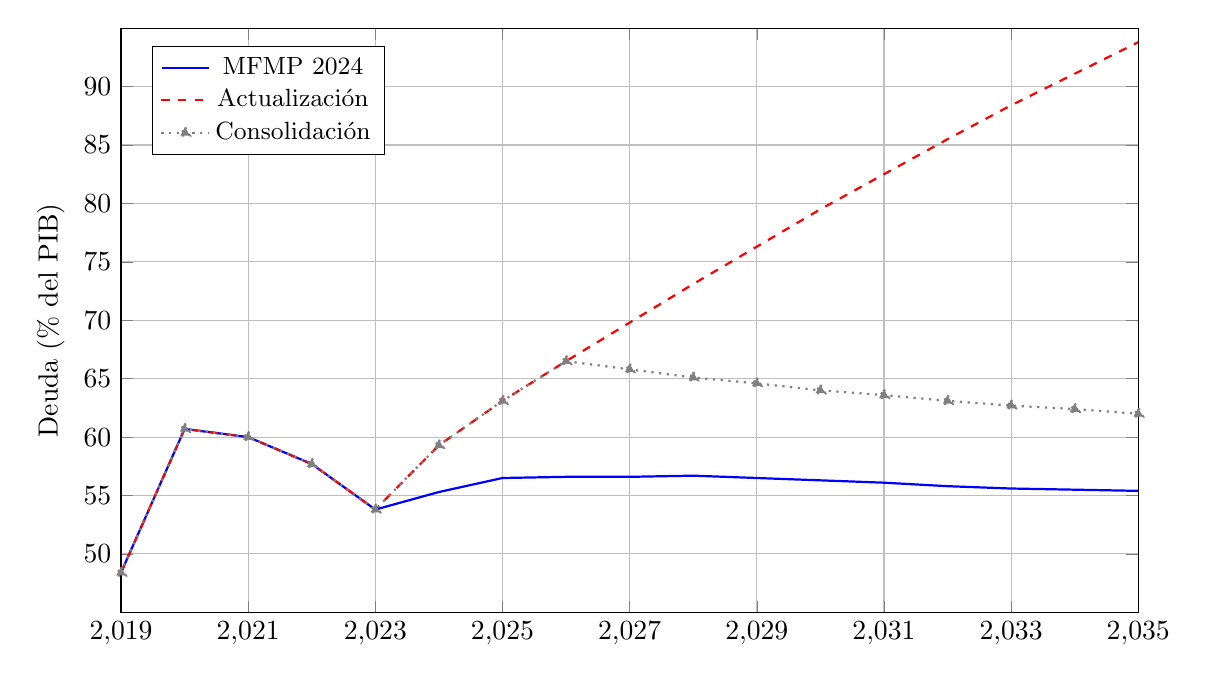
\begin{tikzpicture}
    \begin{axis}[
        width=14.5cm, height=9cm,
%        xlabel={A\~{n}o},
        ylabel={Deuda (\% del PIB)},
        xmin=2019, xmax=2035,
        ymin=45, ymax=95,
        xtick={2019,2021,...,2035},
%        xticklabel style={rotate=90,anchor=east},
        ytick={50,55,...,90},
        legend pos=north west,
        grid=major,
        legend style={font=\small}
    ]

    % Deuda MFMP 2024
    \addplot[
        color=blue, thick
    ] coordinates {
        (2019,48.4) (2020,60.7) (2021,60.0) (2022,57.7) (2023,53.8) 
        (2024,55.3) (2025,56.5) (2026,56.6) (2027,56.6) (2028,56.7) 
        (2029,56.5) (2030,56.3) (2031,56.1) (2032,55.8) (2033,55.6) 
        (2034,55.5) (2035,55.4)
    };
    \addlegendentry{MFMP 2024}

    % Deuda Actualizada
    \addplot[
        color=red, thick, dashed
    ] coordinates {
        (2019,48.4) (2020,60.7) (2021,60.0) (2022,57.7) (2023,53.8) 
        (2024,59.3) (2025,63.1) (2026,66.5) (2027,69.8) (2028,73.1) 
        (2029,76.3) (2030,79.5) (2031,82.5) (2032,85.5) (2033,88.4) 
        (2034,91.1) (2035,93.8) 
    };
    \addlegendentry{Actualizaci\'on}

    % Deuda Consolidación
    \addplot[mark=triangle*, color=gray, thick, dotted ] coordinates {
        (2019,48.4) (2020,60.7) (2021,60.0) (2022,57.7) (2023,53.8) 
        (2024,59.3) (2025,63.1) (2026,66.5) (2027,65.8) (2028,65.1) 
        (2029,64.6) (2030,64.0) (2031,63.6) (2032,63.1) (2033,62.7) 
        (2034,62.4) (2035,62.0) 
    };
    \addlegendentry{Consolidaci\'on}

    \end{axis}
\end{tikzpicture}
%\vspace{0.1cm}
\par\footnotesize{\textit{Fuente: Elaboración propia con base en MFMP 2024, Balance General del GNC y Deuda del GNC, Ministerio de Hacienda.}}
\end{figure}